% Figure for 02_datasets.qmd, copied from slides/AE_week01_Intro/AE_w01_intro.tex.
% Compile with pdflatex, then convert: pdftocairo -svg <name>.pdf ../<name>.svg
\documentclass[class=extarticle, 9pt, tikz, border=4pt]{standalone}
\usepackage[T1]{fontenc}
\renewcommand{\familydefault}{\sfdefault}
\definecolor{PelloGrayDark}{RGB}{60,60,60}
\definecolor{PelloGray}{RGB}{120,120,120}
\definecolor{PelloGrayLight}{RGB}{235,235,235}
\definecolor{PelloGrayUltraLight}{RGB}{248,248,248}
\begin{document}
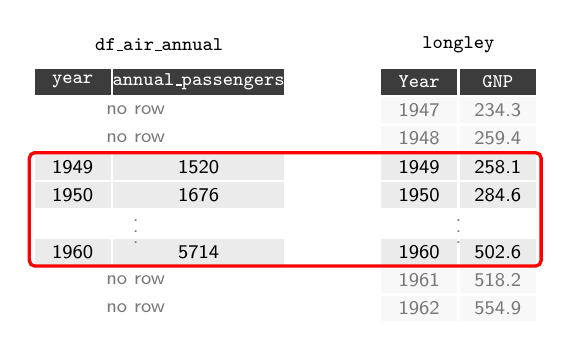
\begin{tikzpicture}[x=1cm, y=0.36cm, font=\scriptsize,
  cell/.style={draw=white, line width=1pt, fill=PelloGrayLight, minimum width=1cm, minimum height=0.36cm, inner sep=0pt},
  wide/.style={cell, minimum width=2.2cm},
  head/.style={fill=PelloGrayDark, text=white, font=\scriptsize\ttfamily},
  gap/.style={text=PelloGray}]
  % table titles
  \node[font=\scriptsize\ttfamily] at (1.1,1.3) {df\_air\_annual};
  \node[font=\scriptsize\ttfamily] at (4.9,1.3) {longley};
  % headers
  \node[cell, head] at (0,0) {year};
  \node[wide, head] at (1.6,0) {annual\_passengers};
  \node[cell, head] at (4.4,0) {Year};
  \node[cell, head] at (5.4,0) {GNP};
  % both ends of the data, aligned by year: df_air_annual covers 1949-1960, longley 1947-1962
  \foreach \r in {1, 2, 7, 8} \node[gap] at (0.8,-\r) {no row};
  \foreach \r/\y/\p in {3/1949/1520, 4/1950/1676, 6/1960/5714} {
    \node[cell] at (0,-\r) {\y};
    \node[wide] at (1.6,-\r) {\p};
  }
  \foreach \r/\y/\g in {3/1949/258.1, 4/1950/284.6, 6/1960/502.6} {
    \node[cell] at (4.4,-\r) {\y};
    \node[cell] at (5.4,-\r) {\g};
  }
  % middle years not shown
  \node[gap] at (0.8,-5) {$\vdots$};
  \node[gap] at (4.9,-5) {$\vdots$};
  % longley years without a match in df_air_annual: dropped by left_join()
  \foreach \r/\y/\g in {1/1947/234.3, 2/1948/259.4, 7/1961/518.2, 8/1962/554.9} {
    \node[cell, fill=PelloGrayUltraLight, text=PelloGray] at (4.4,-\r) {\y};
    \node[cell, fill=PelloGrayUltraLight, text=PelloGray] at (5.4,-\r) {\g};
  }
  % every row of df_air_annual: kept by left_join()
  \draw[red, line width=1.2pt, rounded corners=2pt] (-0.55,-2.5) rectangle (5.95,-6.5);
\end{tikzpicture}
\end{document}
